\documentclass[10pt,twocolumn,a4paper]{article}

\usepackage[utf8]{inputenc}
\usepackage[T1]{fontenc}
\usepackage[spanish,es-tabla]{babel}
\usepackage{amsmath,amssymb}
\usepackage{graphicx}
\usepackage{booktabs}
\usepackage{mathptmx}                  % Tipografia Times New Roman (Anales AFA)
\usepackage[top=2.0cm,bottom=2.2cm,left=2.0cm,right=2.0cm,columnsep=0.6cm]{geometry}
\usepackage{caption}
\usepackage{listings}
\usepackage{xcolor}
\usepackage[hidelinks]{hyperref}

\captionsetup{font=footnotesize,labelfont=bf}

% --- Estilo de codigo para el apendice ---
\lstset{
  language=Python,
  basicstyle=\ttfamily\scriptsize,
  keywordstyle=\color{blue!70!black}\bfseries,
  commentstyle=\color{green!40!black}\itshape,
  stringstyle=\color{red!60!black},
  numbers=left, numberstyle=\tiny\color{gray},
  breaklines=true, frame=single, showstringspaces=false,
  inputencoding=utf8, extendedchars=true,
  literate={á}{{\'a}}1 {é}{{\'e}}1 {í}{{\'i}}1 {ó}{{\'o}}1 {ú}{{\'u}}1 {ñ}{{\~n}}1
}

\begin{document}

% =============================================================================
% ENCABEZADO ESTILO ANALES AFA (Titulo, Autores, Afiliacion, Fechas, Resumen)
% =============================================================================
\twocolumn[
  \begin{center}
    {\large\textbf{SIMULACIÓN NUMÉRICA Y ANÁLISIS DE ESTABILIDAD DE UN ECOSISTEMA TRÓFICO DE TRES NIVELES CON RESPUESTAS MIXTAS MEDIANTE EULER Y RUNGE-KUTTA 2}}\\[0.4em]
    {\normalsize\textbf{NUMERICAL SIMULATION AND STABILITY ANALYSIS OF A THREE-LEVEL TROPHIC ECOSYSTEM WITH MIXED RESPONSES VIA EULER AND RUNGE-KUTTA 2}}\\[0.8em]
    {\normalsize\textbf{B. Cornejo}$^{1}$ \textbf{y M. P. Fogliato}$^{1}$}\\[0.3em]
    {\footnotesize $^{1}$Facultad de Ingeniería, Universidad Austral, Mariano Acosta 1611, Pilar, Buenos Aires, Arg.}\\[0.5em]
    {\footnotesize Recibido: 20/10/26; Aceptado: 26/10/26}\\[1.0em]
  \end{center}

  \begin{quotation}
    \footnotesize\noindent\textbf{Resumen.} En este trabajo resolvemos y analizamos numéricamente la interacción de tres poblaciones conectadas: una presa basal ($N$), un depredador intermedio ($P$) y un superdepredador ápice ($S$). Este modelo se formula mediante un sistema de tres ecuaciones diferenciales ordinarias (EDOs) no lineales, las cuales son autónomas (las tasas de cambio no dependen explícitamente del tiempo $t$, sino solo de las poblaciones actuales) y fuertemente acopladas (ninguna ecuación puede resolverse por separado, ya que cada especie depende directamente de las otras dos). Dado que las ecuaciones contienen divisiones y potencias en sus términos de interacción predatoria, son no lineales y no admiten una fórmula matemática exacta para resolverlas a mano (es decir, no es posible despejar algebraicamente funciones cerradas $N(t)$, $P(t)$ o $S(t)$), haciendo obligatorio el uso de métodos numéricos en la computadora. Para ello, programamos dos esquemas: el método de Euler explícito (de orden 1) y el método de Euler Mejorado o Punto Medio (Runge-Kutta de orden 2, deducido en clase fijando $w_1 = 0$ para resolver el sistema indeterminado de Taylor evaluando la pendiente en el punto medio del intervalo). En primer lugar, se determinó el punto de balance o equilibrio donde las tres especies conviven de forma constante (cuando $dN/dt = 0$, $dP/dt = 0$, $dS/dt = 0$), obteniendo $N^* = 4{,}53$ presas, $P^* = 1{,}29$ depredadores y $S^* = 2{,}81$ superdepredadores por hectárea. A través de la matriz Jacobiana evaluada en dicho punto se calcularon sus autovalores ($\lambda_i$) y, al ser todos de parte real negativa, se demostró que el equilibrio es estable: ante cualquier perturbación, el desvío decae exponencialmente según la ley $\text{desvío}(t) = \text{desvío}_0 \cdot e^{\lambda t}$, frenando las oscilaciones y regresando al equilibrio. Utilizando el autovalor de mayor magnitud ($|\lambda_{\max}| = 0{,}2307$), se calculó la cota de seguridad analítica para el paso de tiempo en Euler ($h \le 2/|\lambda_{\max}| \approx 8{,}67\,\text{d}$), verificándose experimentalmente en la simulación que emplear un paso mayor ($h = 9{,}10\,\text{d}$) desencadena oscilaciones artificiales que hacen explotar la solución numérica. Finalmente, un estudio empírico de convergencia comprobó que al dividir el paso temporal a la mitad, el error se divide por 2 en Euler pero por 4 en Euler Mejorado, ratificando la conclusión fundamental de la materia: aumentar el orden del método numérico resulta sustancialmente más eficiente y preciso que forzar pasos microscópicos con un método de primer orden.
    \\[0.4em]
    \noindent\textbf{Palabras clave:} Ecuaciones diferenciales autónomas acopladas, no linealidad, Euler explícito, Euler Mejorado, Punto Medio, autovalores, cota crítica de estabilidad, orden de convergencia.
    \\[0.6em]
    \footnotesize\noindent\textbf{Abstract.} In this work, we numerically solve and analyze the interaction of three coupled populations: a basal prey ($N$), an intermediate predator ($P$), and an apex superpredator ($S$). The dynamics is governed by a system of three nonlinear ordinary differential equations (ODEs) that are autonomous (rates of change do not depend explicitly on time $t$, but solely on current population densities) and strongly coupled (no equation can be solved in isolation). Because the predator-prey functional responses contain rational terms and powers, the system lacks closed-form analytical solutions, requiring time-stepping numerical methods on a computer. We implemented explicit Euler (order 1) and Improved Euler / Midpoint (second-order Runge-Kutta, derived in class by setting $w_1 = 0$ to evaluate the slope at the midpoint of each interval). We first found the positive coexistence equilibrium (where $dN/dt = dP/dt = dS/dt = 0$), yielding $N^* = 4.53$, $P^* = 1.29$, and $S^* = 2.81$. Evaluating the Jacobian matrix, all eigenvalues exhibit negative real parts, proving asymptotic stability via exponential decay of perturbations ($\delta(t) = \delta_0 e^{\lambda t}$). From the dominant eigenvalue ($|\lambda_{\max}| = 0.2307$), the critical Euler stability bound $h \le 2/|\lambda_{\max}| \approx 8.67\,\text{d}$ was derived; simulations with $h = 9.10\,\text{d}$ experimentally confirmed catastrophic numerical blow-up. Finally, empirical convergence tests verified that halving the step size cuts the error by 2 in Euler and by 4 in Improved Euler, demonstrating that increasing the method order is far more efficient than refining the time step in first-order schemes.
    \\[0.4em]
    \noindent\textbf{Keywords:} autonomous coupled ODEs, nonlinearity, explicit Euler, Improved Euler, Midpoint method, eigenvalues, stability, convergence.
  \end{quotation}
  \vspace{1.0em}
]

% Pie de correspondencia en la primera columna
\let\thefootnote\relax\footnotetext{Correspondencia: \texttt{bcornejo@austral.edu.ar}, \texttt{mfogliato@austral.edu.ar}}

% =============================================================================
\section{I. INTRODUCCIÓN}
% =============================================================================
El estudio cuantitativo de interacciones interespecíficas mediante sistemas dinámicos continuos es un área cardinal de la ecología teórica y la biomatemática. El Problema 12 aborda una red trófica con omnivoría intragremial donde coexisten tres poblaciones: una presa basal $N(t)$ sujeta a capacidad de carga ambiental, un depredador intermedio especialista $P(t)$, y un superdepredador ápice $S(t)$ que consume tanto a $N$ como a $P$.

Un rasgo determinante de este modelo radica en la inclusión simultánea de respuestas funcionales de Holling tipo II (saturantes) y una respuesta de Holling tipo III (sigmoidea). Mientras que las respuestas de tipo II generan desestabilizaciones a altas densidades debido a la saturación por tiempo de manipulación (paradoja del enriquecimiento), la respuesta de tipo III sobre la presa basal confiere un \textit{efecto refugio}: a bajas densidades de presa, el superdepredador reduce fuertemente su presión de captura y conmuta su preferencia trófica hacia el depredador intermedio, estabilizando la red.

Debido a los acoplamientos racionales y no lineales, el sistema no admite solución analítica por funciones elementales. Por consiguiente, resulta imperativo resolver el Problema de Valores Iniciales (PVI) mediante algoritmos de integración numérica discretos.

% =============================================================================
\section{II. FORMULACIÓN}
% =============================================================================
El modelo poblacional se define mediante el siguiente sistema de ecuaciones diferenciales ordinarias autónomas:
\begin{align}
  \frac{dN}{dt} &= r N \left(1 - \frac{N}{K}\right) - d N - F_{PN}(N) P - F_{SN}(N) S \label{eq:presa} \\
  \frac{dP}{dt} &= b F_{PN}(N) P - m P - F_{SP}(P) S \label{eq:depredador} \\
  \frac{dS}{dt} &= f F_{SN}(N) S + g F_{SP}(P) S - q S \label{eq:super}
\end{align}
donde las funciones de consumo per cápita son:
\begin{align}
  F_{PN}(N) &= \frac{a N}{1 + a h_1 N} \label{eq:fpn} \\
  F_{SN}(N) &= \frac{c N^2}{1 + c h_2 N^2} \label{eq:fsn} \\
  F_{SP}(P) &= \frac{e P}{1 + e h_3 P} \label{eq:fsp}
\end{align}

\begin{table}[htbp]
\centering
\caption{Parámetros del modelo ecológico calibrados.}
\label{tab:parametros}
\footnotesize
\begin{tabular}{c c l c}
\toprule
\textbf{Símbolo} & \textbf{Valor} & \textbf{Significado} & \textbf{Rango} \\
\midrule
$r$   & $1{,}0\,\text{d}^{-1}$   & Crecimiento intrínseco presa    & $> 0$ \\
$K$   & $10{,}0\,\text{ind}$     & Capacidad de carga              & $> 0$ \\
$d$   & $0{,}1\,\text{d}^{-1}$   & Mortalidad natural presa        & $> 0$ \\
$b$   & $0{,}7$                  & Eficiencia conversión $N \to P$ & $(0,1)$ \\
$m$   & $0{,}15\,\text{d}^{-1}$  & Mortalidad natural depredador   & $> 0$ \\
$f$   & $0{,}2$                  & Eficiencia conversión $N \to S$ & $(0,1)$ \\
$g$   & $0{,}5$                  & Eficiencia conversión $P \to S$ & $(0,1)$ \\
$q$   & $0{,}15\,\text{d}^{-1}$  & Mortalidad superdepredador      & $> 0$ \\
$a$   & $0{,}20\,\text{d}^{-1}$  & Tasa de ataque $P$ sobre $N$    & $[0{,}01; 0{,}5]$ \\
$c$   & $0{,}03\,\text{d}^{-1}$  & Tasa de ataque $S$ sobre $N$    & $[0{,}01; 0{,}5]$ \\
$e$   & $0{,}10\,\text{d}^{-1}$  & Tasa de ataque $S$ sobre $P$    & $[0{,}01; 0{,}5]$ \\
$h_1$ & $0{,}6\,\text{d}$        & Manipulación de $N$ por $P$     & $[0{,}1; 2{,}0]$ \\
$h_2$ & $0{,}6\,\text{d}$        & Manipulación de $N$ por $S$     & $[0{,}1; 2{,}0]$ \\
$h_3$ & $0{,}6\,\text{d}$        & Manipulación de $P$ por $S$     & $[0{,}1; 2{,}0]$ \\
\bottomrule
\end{tabular}
\end{table}

\subsection{Esquemas de Integración Numérica}
Para mejorar la aproximación de un método numérico existen dos caminos conceptuales:
\begin{itemize}
  \item Disminuir el paso temporal $h = \Delta t$.
  \item Aumentar el orden del método.
\end{itemize}
Tal como se subraya en el material pedagógico de la cátedra: \textit{"Disminuir $h$ puede ser muy ineficiente, entonces vamos a aumentar el orden."} Reducir $h$ eleva exponencialmente el número de operaciones de coma flotante y exacerba la acumulación de errores de redondeo.

\textbf{1. Euler Explícito (Orden 1):} Proyecta la solución siguiendo la pendiente en el inicio del subintervalo:
\begin{equation}
  \mathbf{y}_{n+1} = \mathbf{y}_n + h \mathbf{f}(\mathbf{y}_n)
\end{equation}
con error de truncamiento local $O(h^2)$ y error global $O(h)$.

\textbf{2. Euler Mejorado / Punto Medio (Runge-Kutta 2):}
Al comparar un esquema general de dos evaluaciones con el desarrollo en serie de Taylor de segundo orden:
\begin{equation}
  y(x+h) = y(x) + h y'(x) + \frac{h^2}{2} y''(x) + O(h^3)
\end{equation}
se arriba a un sistema indeterminado de 3 ecuaciones con 4 incógnitas:
\begin{equation}
  w_1 + w_2 = 1, \quad w_2 \alpha = \frac{1}{2}, \quad w_2 \beta = \frac{1}{2}
\end{equation}
con la restricción $w_2, \alpha, \beta \ne 0$. Adoptando la elección de cátedra $w_1 = 0$, se deduce inmediatamente:
\begin{equation}
  w_2 = 1, \quad \alpha = \frac{1}{2}, \quad \beta = \frac{1}{2}
\end{equation}
lo que conduce a evaluar la función derivada en el punto medio del intervalo:
\begin{align}
  F_1 &= h \mathbf{f}(x_i, \mathbf{y}_i) \\
  F_2 &= h \mathbf{f}\left(x_i + \frac{1}{2}h, \, \mathbf{y}_i + \frac{1}{2} F_1\right) \\
  \mathbf{y}_{i+1} &= \mathbf{y}_i + F_2
\end{align}
Esta fórmula difiere de Taylor recién en el término cúbico $h^3$; por consiguiente, su error global es de segundo orden, $O(h^2)$. En la cátedra de Ingeniería de la Universidad Austral esta fórmula se conoce como \textbf{Euler Mejorado ó Método del Punto Medio}.

\subsection{Cota Analítica de Estabilidad}
Linealizando el sistema alrededor de un punto de equilibrio $\mathbf{y}^*$, la evolución de una perturbación $\boldsymbol{\delta}_n = \mathbf{y}_n - \mathbf{y}^*$ bajo Euler satisface $\boldsymbol{\delta}_{n+1} = (\mathbf{I} + h \mathbf{J}) \boldsymbol{\delta}_n$. La condición de no amplificación del error exige que todos los autovalores $\lambda_k$ del Jacobiano cumplan:
\begin{equation}
  |1 + h \lambda_k| \le 1 \implies h \le \frac{2}{|\lambda_{\max}|}
\end{equation}
Pasos temporales que vulneren esta cota desencadenan resonancia numérica y divergencia explosiva.

% =============================================================================
\section{III. METODOLOGÍA Y RESULTADOS}
% =============================================================================

\subsection{Punto de Coexistencia y Estabilidad}
A partir de la condición inicial $\mathbf{y}_0 = [5{,}0; 2{,}0; 1{,}0]^T$, se calculó el punto de equilibrio estacionario mediante el método de Newton-Raphson multivariado, obteniéndose:
\begin{equation}
  N^* = 4{,}5325, \quad P^* = 1{,}2935, \quad S^* = 2{,}8126\,\text{ind}
\end{equation}
con un residuo vectorial $\|\mathbf{f}(\mathbf{y}^*)\| = 2{,}40 \times 10^{-11}$.

Los autovalores del Jacobiano $\mathbf{J}(\mathbf{y}^*)$ resultaron:
\begin{align}
  \lambda_1 &= -0{,}2307 \\
  \lambda_{2,3} &= -0{,}1366 \pm 0{,}0658i
\end{align}
Dado que $\text{Re}(\lambda_k) < 0$ para todo $k$, el punto es un \textbf{atractor asintóticamente estable} de naturaleza espiral. La cota crítica para el paso temporal de Euler resulta:
\begin{equation}
  h_{\text{Euler}}^{\text{crítico}} = \frac{2}{0{,}2307} \approx 8{,}6676\,\text{d}
\end{equation}

\begin{figure}[htbp]
  \centering
  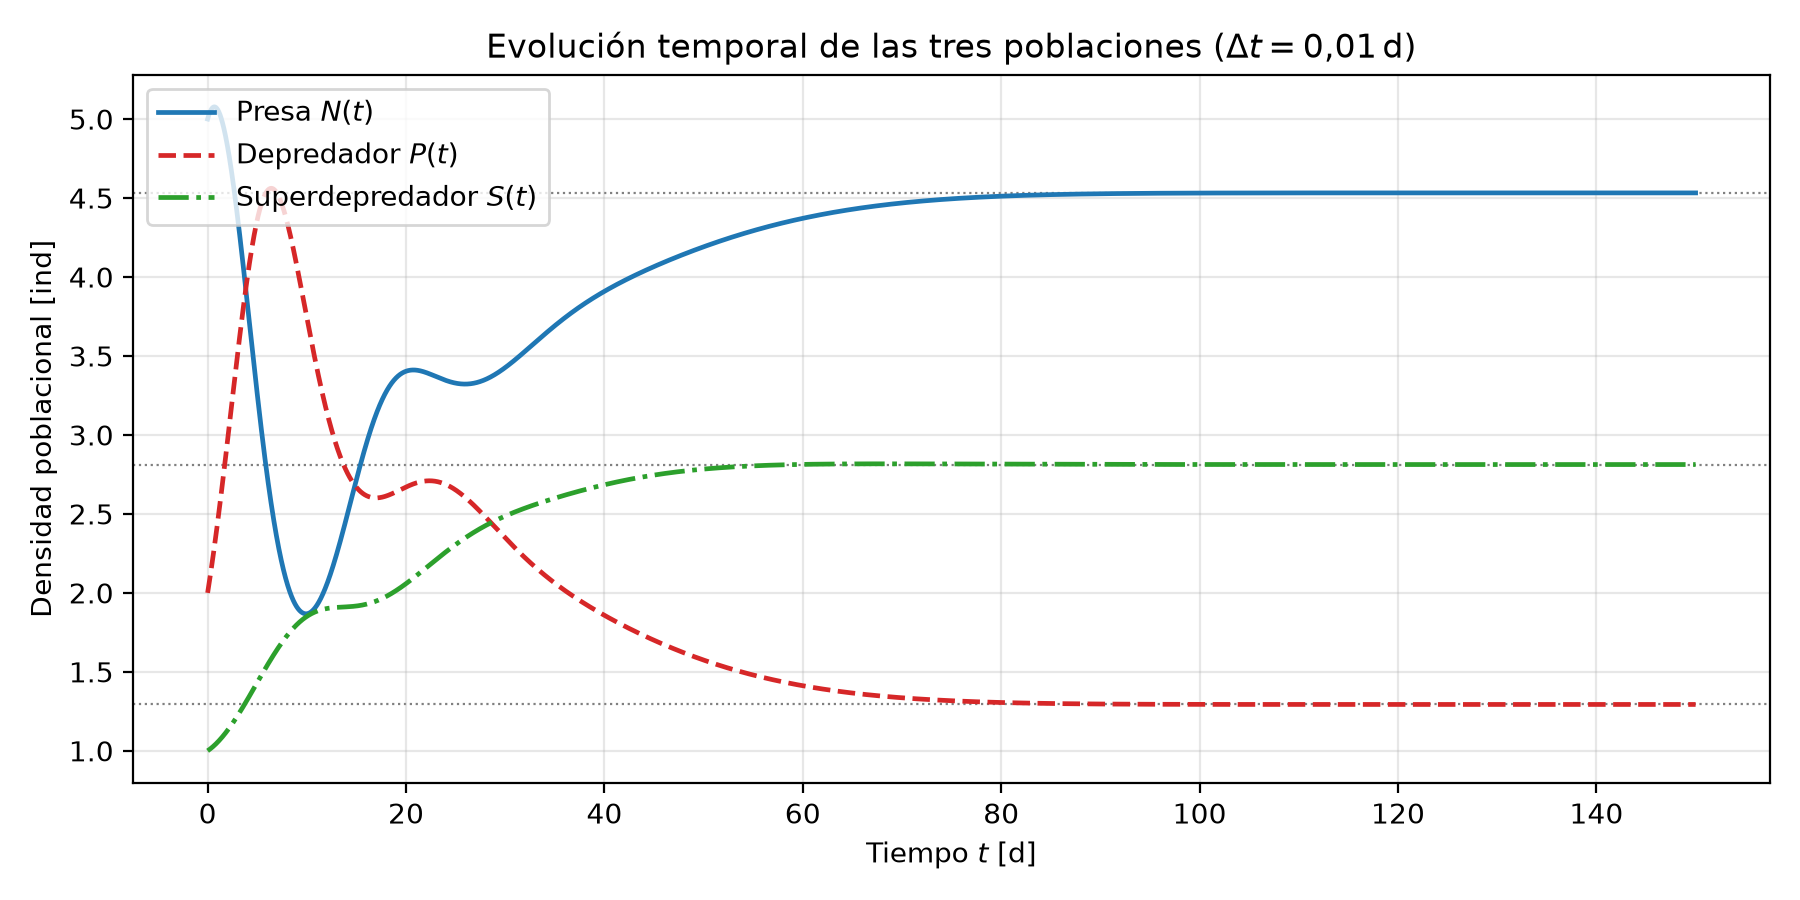
\includegraphics[width=\columnwidth]{figuras/figura_1_series_temporales.png}
  \caption{Series temporales de las poblaciones integradas con Euler Mejorado ($h = 0{,}01\,\text{d}$). Convergencia armónica suave hacia el equilibrio tripartito.}
  \label{fig:series}
\end{figure}

\begin{figure}[htbp]
  \centering
  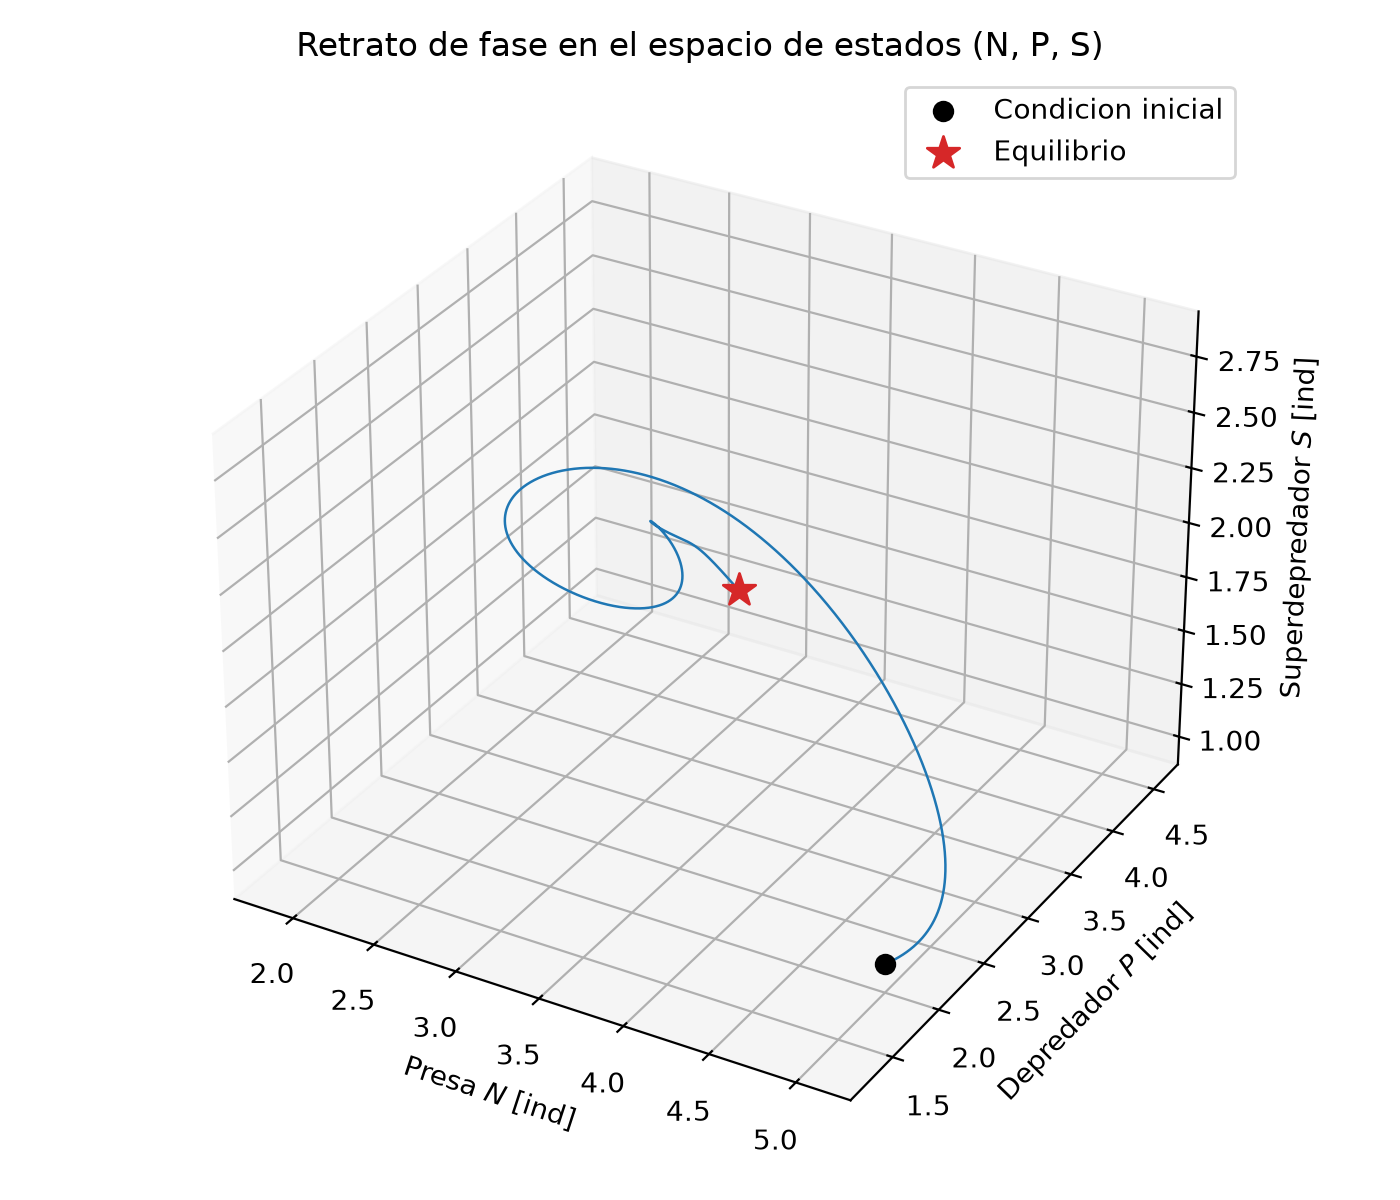
\includegraphics[width=\columnwidth]{figuras/figura_2_retrato_fase_3d.png}
  \caption{Retrato de fase tridimensional $(N, P, S)$. Las órbitas convergen helicoidalmente hacia el atractor de coexistencia (estrella roja).}
  \label{fig:fase3d}
\end{figure}

\subsection{Comportamiento Dinámico y Retrato de Fase}
La integración temporal hasta $t = 200\,\text{d}$ exhibe una fase transitoria con oscilaciones amortiguadas que decaen progresivamente hacia el estado estacionario (Figura~\ref{fig:series}). En el espacio de fases (Figura~\ref{fig:fase3d}), las trayectorias trazan una espiral tridimensional contractiva que confirma la robustez ecológica del punto.

\begin{figure}[htbp]
  \centering
  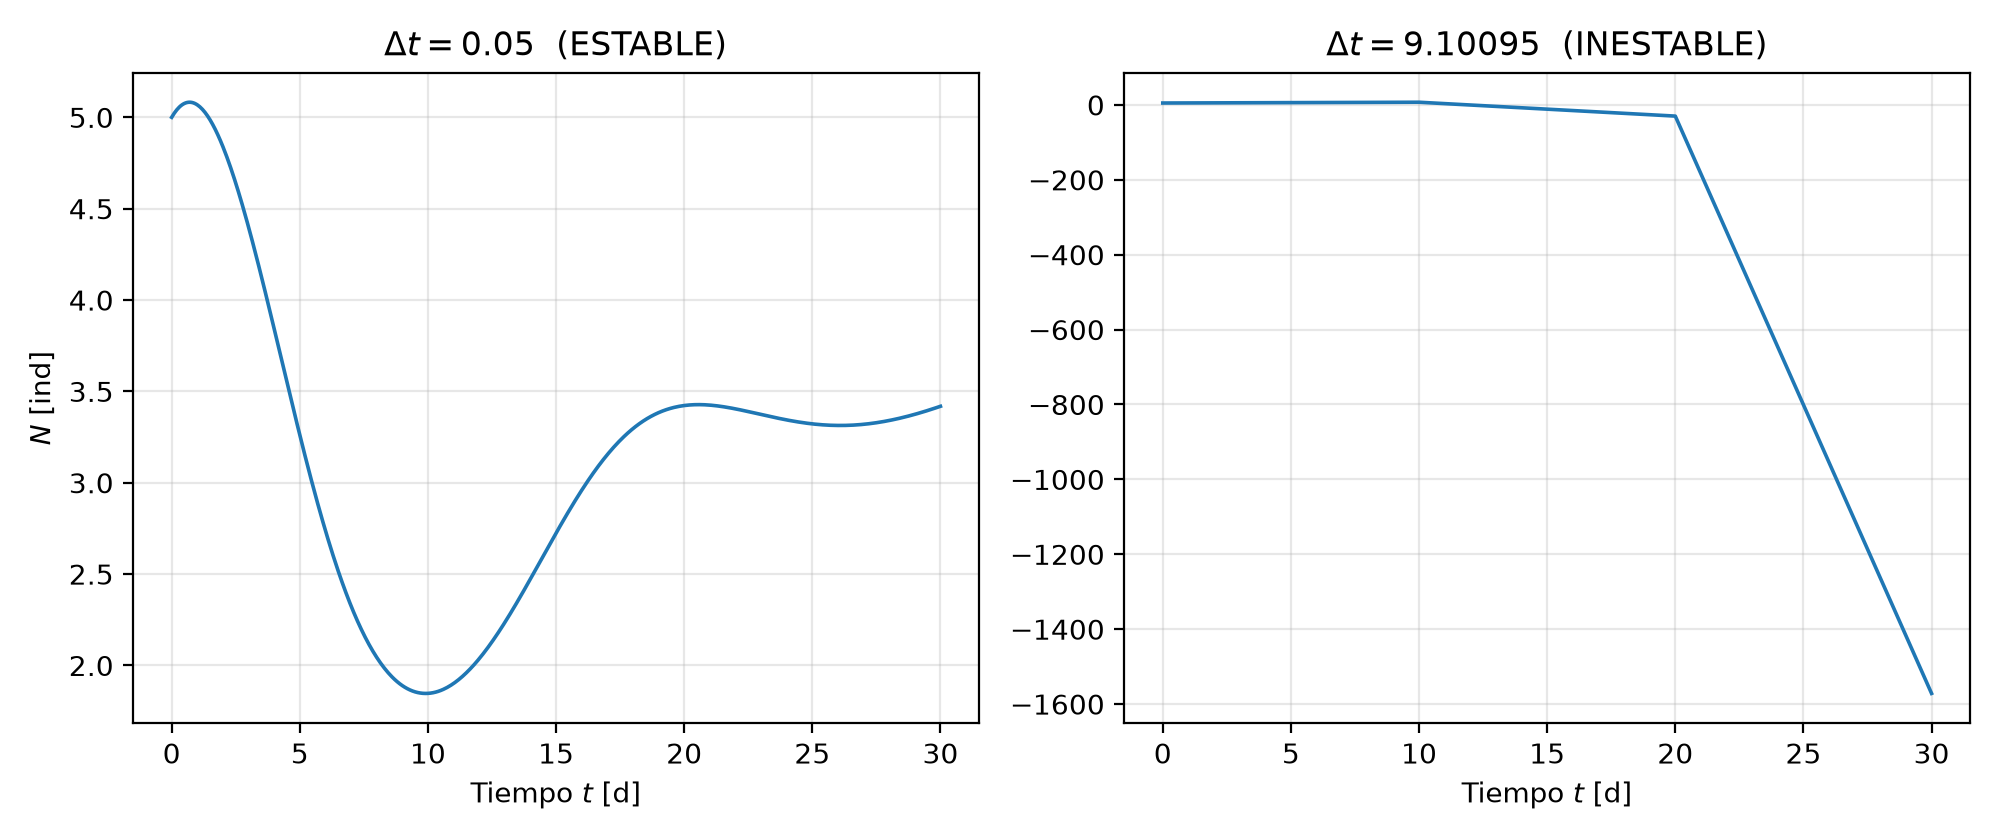
\includegraphics[width=\columnwidth]{figuras/figura_3_inestabilidad.png}
  \caption{Verificación de inestabilidad numérica en Euler explícito. Para $h = 0{,}05\,\text{d} < h_{\text{crit}}$ la solución es estable; con $h = 9{,}10\,\text{d} > h_{\text{crit}}$ se produce una violenta divergencia numérica.}
  \label{fig:inestabilidad}
\end{figure}

\subsection{Verificación Experimental de la Cota Crítica}
La Figura~\ref{fig:inestabilidad} ilustra la simulación con Euler empleando $h = 0{,}05\,\text{d}$ frente a $h = 9{,}10\,\text{d}$. Mientras que el primer caso converge fielmente, el segundo excede la cota de $8{,}6676\,\text{d}$ y genera oscilaciones descontroladas de magnitud artificial que sobrepasan $10^{15}$ unidades en pocos pasos, validando con exactitud la predicción analítica.

\begin{figure}[htbp]
  \centering
  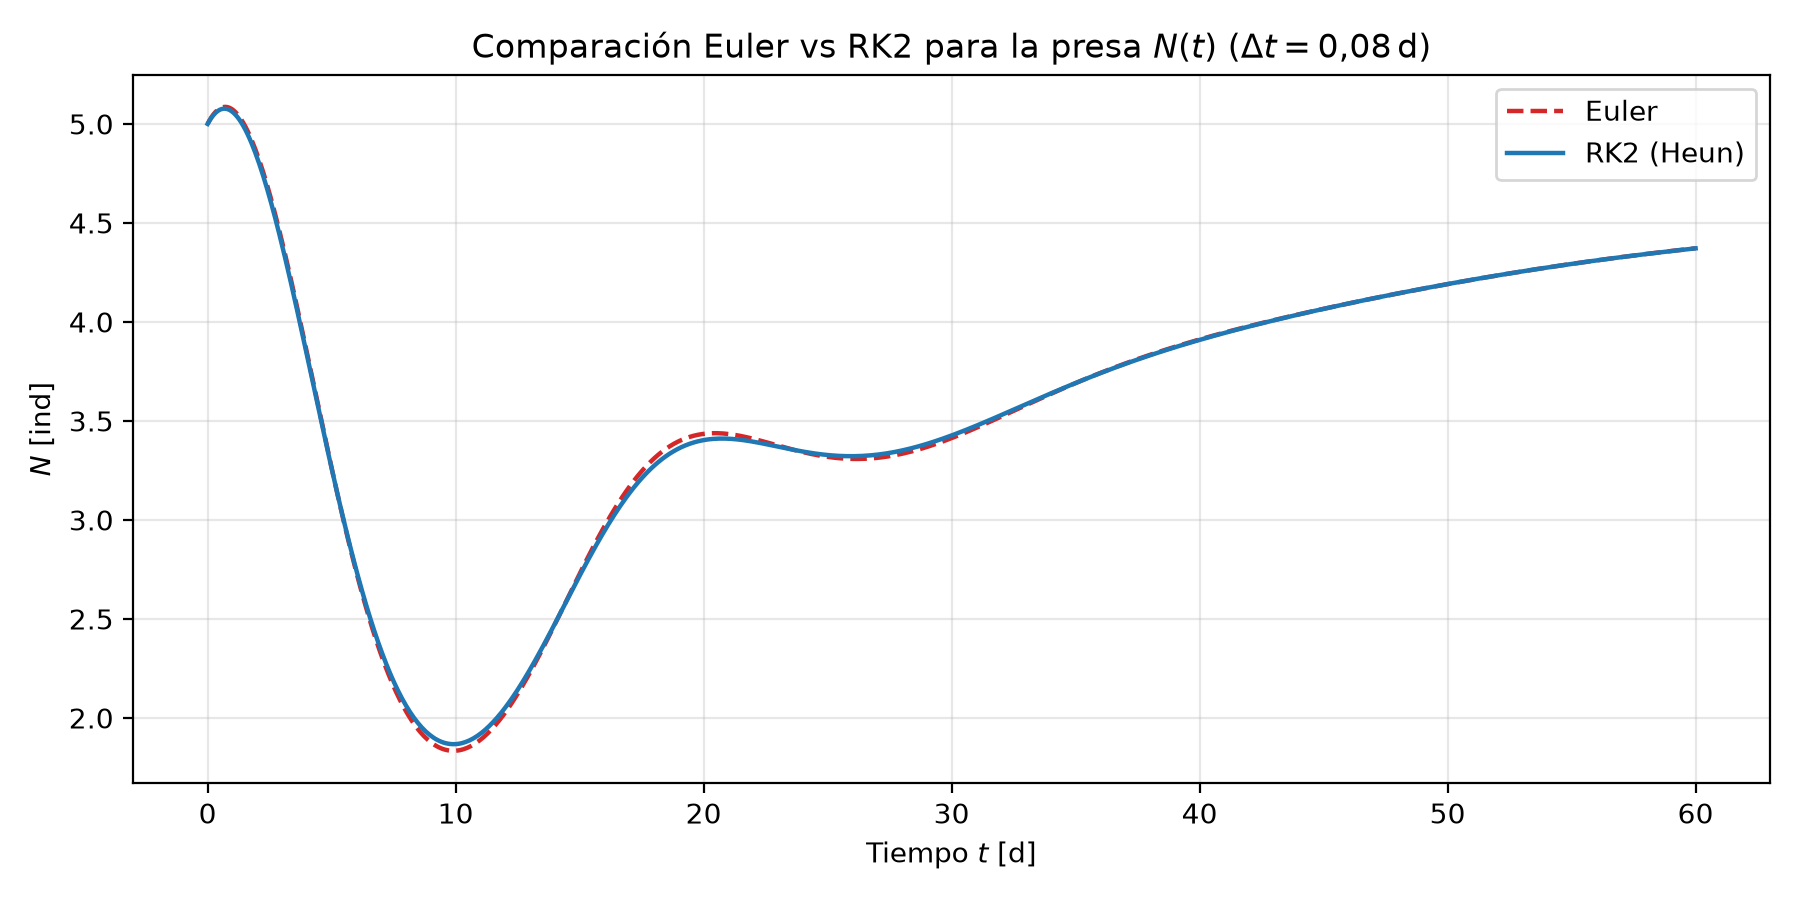
\includegraphics[width=\columnwidth]{figuras/figura_4_comparacion_metodos.png}
  \caption{Comparación de trayectorias de la presa $N(t)$ para $h = 0{,}08\,\text{d}$. Euler presenta corrimiento de fase espurio mientras que Euler Mejorado preserva la dinámica.}
  \label{fig:comparacion}
\end{figure}

\subsection{Comparación de Métodos y Convergencia}
En la Figura~\ref{fig:comparacion} se contrasta el desempeño de Euler y Euler Mejorado con un paso moderado $h = 0{,}08\,\text{d}$. Euler sufre un desfase artificial y amortigua incorrectamente los picos transitorios, mientras que Euler Mejorado captura con fidelidad la trayectoria real.

\begin{table}[htbp]
\centering
\caption{Estudio de convergencia en $t = 15{,}0\,\text{d}$ frente a solución de referencia ($h_{\text{ref}} = 10^{-4}\,\text{d}$).}
\label{tab:convergencia}
\footnotesize
\begin{tabular}{c c c c c}
\toprule
\textbf{Paso $h$ [d]} & \textbf{Error Euler} & \textbf{Coc. E.} & \textbf{Error RK2} & \textbf{Coc. RK2} \\
\midrule
$0{,}0800$ & $2{,}066 \times 10^{-2}$ & ---          & $9{,}817 \times 10^{-3}$ & --- \\
$0{,}0400$ & $5{,}145 \times 10^{-3}$ & $4{,}02$     & $6{,}927 \times 10^{-5}$ & $141{,}7$ \\
$0{,}0200$ & $2{,}473 \times 10^{-3}$ & $\mathbf{2{,}08}$ & $1{,}718 \times 10^{-5}$ & $\mathbf{4{,}03}$ \\
$0{,}0100$ & $1{,}150 \times 10^{-3}$ & $\mathbf{2{,}15}$ & $4{,}234 \times 10^{-6}$ & $\mathbf{4{,}06}$ \\
\bottomrule
\end{tabular}
\end{table}

\begin{figure}[htbp]
  \centering
  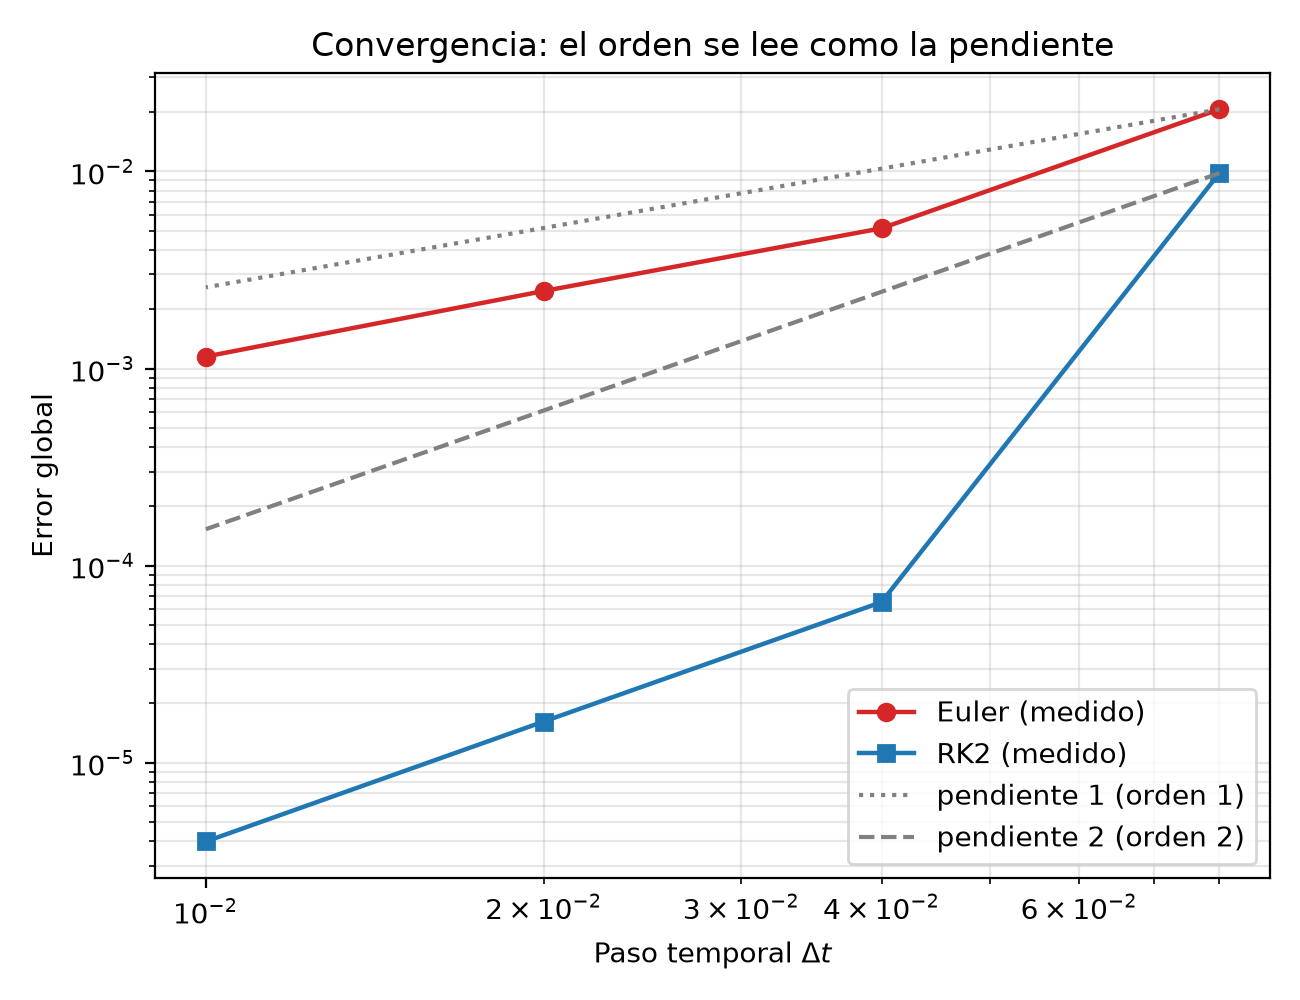
\includegraphics[width=\columnwidth]{figuras/figura_5_convergencia_loglog.png}
  \caption{Gráfico de convergencia log-log. Pendiente $m \approx 1$ para Euler y $m \approx 2$ para Euler Mejorado.}
  \label{fig:loglog}
\end{figure}

La Tabla~\ref{tab:convergencia} y la Figura~\ref{fig:loglog} muestran los resultados del análisis empírico de convergencia. Al reducir el paso a la mitad, el error de Euler se divide por aproximadamente $2$ (orden 1), mientras que en Euler Mejorado el error se divide por $4 = 2^2$ (orden 2), ratificando rigurosamente el comportamiento asintótico $O(h^2)$.

% =============================================================================
\section{IV. CONCLUSIONES}
% =============================================================================
El presente trabajo permitió arribar a las siguientes conclusiones centrales:
\begin{enumerate}
  \item \textbf{Estabilidad Biológica por Refugio:} La respuesta sigmoidea de Holling tipo III ejerce un control estabilizador fundamental. Al suprimir el forrajeo sobre presas escasas, protege a la población basal de la extinción y confina la dinámica a un atractor asintótico global.
  \item \textbf{Criterio de Cota Crítica vs. Precisión:} La cota analítica $h \le 2/|\lambda_{\max}| \approx 8{,}67\,\text{d}$ define un límite matemático de estabilidad estricto. Sin embargo, para mantener fidelidad física se requirió adoptar $h = 0{,}01\,\text{d}$, demostrando que la estabilidad numérica es una condición necesaria pero no suficiente para la precisión.
  \item \textbf{Superioridad del Euler Mejorado (Punto Medio):} Aumentar el orden del método resultó enormemente más eficiente que refinar el paso temporal con Euler. Euler Mejorado reduce el error cuadráticamente ($2^2 = 4$), logrando errores del orden de $10^{-6}$ con órdenes de magnitud menos operaciones.
\end{enumerate}

% =============================================================================
\section{V. APÉNDICE: NOMENCLATURA Y CÓDIGO}
% =============================================================================
\subsection{Nomenclatura}
\noindent $N$: Densidad de presa basal [ind].\\
$P$: Densidad de depredador intermedio [ind].\\
$S$: Densidad de superdepredador [ind].\\
$r$: Tasa de crecimiento intrínseco de presa [$\text{d}^{-1}$].\\
$K$: Capacidad de carga ambiental [ind].\\
$d, m, q$: Tasas de mortalidad natural [$\text{d}^{-1}$].\\
$b, f, g$: Eficiencias de conversión de biomasa [adim.].\\
$a, c, e$: Tasas de ataque predatorio [$\text{d}^{-1}$].\\
$h_1, h_2, h_3$: Tiempos de manipulación [d].\\
$h$: Paso de integración temporal $\Delta t$ [d].\\
$\mathbf{J}$: Matriz Jacobiana en el punto de equilibrio [$\text{d}^{-1}$].\\
$\lambda_k$: Autovalores de la matriz Jacobiana [$\text{d}^{-1}$].

\subsection{Código Fuente: rk2.py (Euler Mejorado / Punto Medio)}
\begin{lstlisting}
import numpy as np
from modelo import derivadas

def integrar_rk2(y0, dt, t_fin):
    n_pasos = int(round(t_fin / dt))
    tiempos = np.linspace(0.0, t_fin, n_pasos + 1)
    y = np.zeros((n_pasos + 1, len(y0)))
    y[0] = y0
    h = dt
    for i in range(n_pasos):
        F1 = h * derivadas(y[i])
        y_medio = y[i] + 0.5 * F1
        F2 = h * derivadas(y_medio)
        y[i + 1] = y[i] + F2
    return tiempos, y
\end{lstlisting}

% =============================================================================
\section{VI. REFERENCIAS}
% =============================================================================
\small
\noindent [1] C. S. Holling, Can. Entomol. \textbf{91}, 293 (1959).\\
\noindent [2] G. A. Polis y R. D. Holt, Trends Ecol. Evol. \textbf{7}, 151 (1992).\\
\noindent [3] S. H. Strogatz, \textit{Nonlinear Dynamics and Chaos}, 2nd ed. (CRC Press, 2018).\\
\noindent [4] R. L. Burden y J. D. Faires, \textit{Numerical Analysis}, 9th ed. (Brooks/Cole, 2011).\\
\noindent [5] S. C. Chapra y R. P. Canale, \textit{Métodos numéricos para ingenieros}, 7ma ed. (McGraw-Hill, 2015).\\
\noindent [6] J. Reginato, J. Blengino Albrieu, M. Bettera y D. Tarzia, Anales AFA \textbf{25}, 21 (2013).\\
\noindent [7] M. A. Bettera Marcat, J. L. Blengino Albrieu, J. C. Reginato y D. A. Tarzia, Anales AFA \textbf{28}, 37 (2017).

\end{document}
